\section{8 bit multiplication \& division}
\subsection{Aim}
To multiply and divide two 8bit numbers

\subsection{Code}
\begin{lstlisting}
ORG 0000

; Multiplying 20H with 10H
MOV A, #20H
MOV B, #10H
MUL AB
MOV R0, B ; Storing upper byte of result
MOV R1, A ; Storing lower byte of result

; Dividing 20H with 10H
MOV A, #20H
MOV B, #10H
DIV AB
MOV R2, B ; Remainder of division
MOV R3, A ; Quotient of division	

END
\end{lstlisting}

\subsection{Output}
\textbf{Input} 20H (R0R1), 10H (R2R3)\\
\textbf{Output}\\
Multiplication: 0200H (R0R1)\\
Division: Remainder - 00 (R2), Quotient - 02H (R3)
\begin{center}
	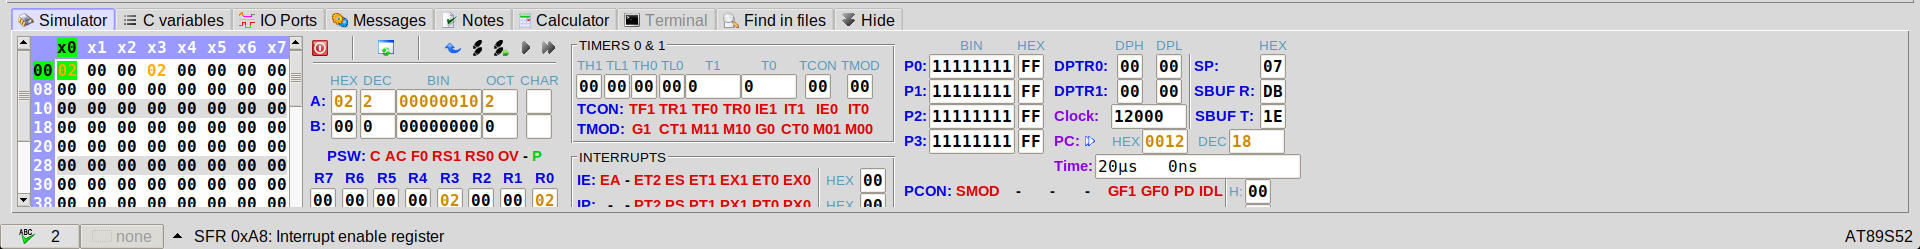
\includegraphics[width=\textwidth]{img/p23.png}
\end{center}

\subsection{Result}
Two 8 bit numbers were multiplied and divided in mcu8051ide